
\section{Maximum Likelihood}
\begin{enumerate}
\item Generate equiprobable $X \in \cbrak{1,-1}$.\\
\solution Refer the below code section,
\begin{lstlisting}
	chapter3/codes/eqi_prob.py
\end{lstlisting}
\item Generate 
\begin{equation}
Y = AX+N,
\end{equation}
where $A = 5$ dB,  and $N \sim \gauss{0}{1}$.\\
\solution Refer the below code section,
\begin{lstlisting}
	chapter3/codes/Y_gau.py
\end{lstlisting}
\item Plot $Y$ using a scatter plot.\\
\solution 
\begin{lstlisting}
		chapter3/codes/scatter.py
\end{lstlisting}
\begin{figure}[H]
\centering
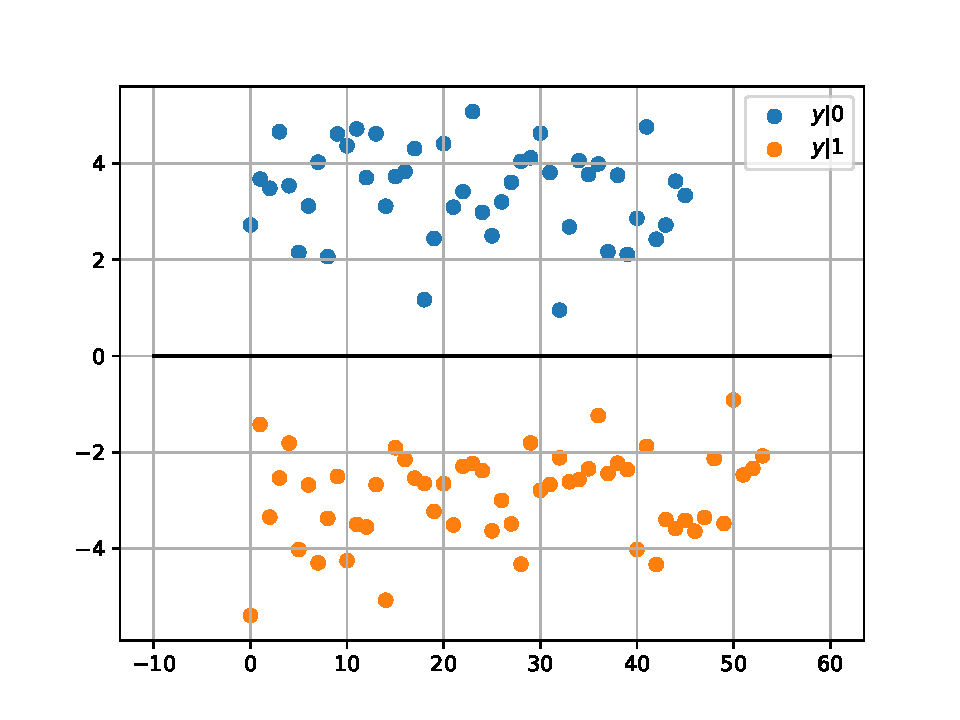
\includegraphics[scale=0.8]{chapter3/figs/bpsk_scatter.pdf}
\caption{Scatter plot of $Y$}
\label{fig:bpsk_scatter}
\end{figure}
\item Guess how to estimate $X$ from $Y$.\\
\solution
According to decision rule 
\begin{equation}
P(Y > y) \\
y \dec{1}{-1} 0
\label{eq:bpsk_decision}
\end{equation}
\item
\label{ml-ch4_sim}
Find 
\begin{equation}
	P_{e|0} = \pr{\hat{X} = -1|X=1}
\end{equation}
and 
\begin{equation}
	P_{e|1} = \pr{\hat{X} = 1|X=-1}
\end{equation}\\

\solution using decision rule in 
\begin{align}
	\pr{\hat{X} = -1|X=1} &= \pr{Y < 0|X=1}&\\
	&= \pr{AX + N < 0|X=1}&\\ 
	&= \pr{A + N < 0}&\\
	&= \pr{N < -A}\\
        &= \pr{N > A}
\end{align}
\begin{align}
	\pr{\hat{X} = 1|X=-1} &= \pr{Y > 0|X=-1}&\\
	&= \pr{N > A}
\end{align}
\begin{align*}
  \pr{N > A}&=\pr{\frac{N-0}{1}> \frac{A-0}{1}}\\&=Q(\frac{A-0}{1})=Q(A)
\end{align*}
\begin{equation}
   P_{e|0} = P_{e|1}=Q(A) = \pr{N > A}
\end{equation}
%
\item Find $P_e$ assuming that $X$ has equiprobable symbols.\\
\solution
\begin{flalign}
	P_e &= \pr{X=1}P_{e|1} + \pr{X=-1}P_{e|0}&\\
	\intertext{Since $X$ is equiprobable}\\
	\label{eq:bpsk_prob_error_equi}
	P_e &= \frac{1}{2}P_{e|1} + \frac{1}{2}P_{e|0}
\end{flalign}
Substituting 
\begin{equation}
	P_e = \pr{N > A}
\end{equation}
Given a random varible $X \sim \gauss{0}{1}$ the Q-function is defined as
\begin{align}
	Q(x) &= \pr{X > x}\\
	\label{eq:q_func_integral}
	Q(x) &= \frac{1}{\sqrt{2\pi}} \int_x^\infty \exp\left(-\frac{u^2}{2}\right) \, du.\\
\end{align}
Using the Q-function, $P_e$ is rewritten as
\begin{equation}
	P_e = Q(A)
\end{equation} 
%
\item
Verify by plotting  the theoretical $P_e$ with respect to $A$ from 0 to 10 dB.\\
\solution 
\begin{lstlisting}
		chapter3/codes/bpsk_pe.py
\end{lstlisting}
\begin{figure}[H]
\centering
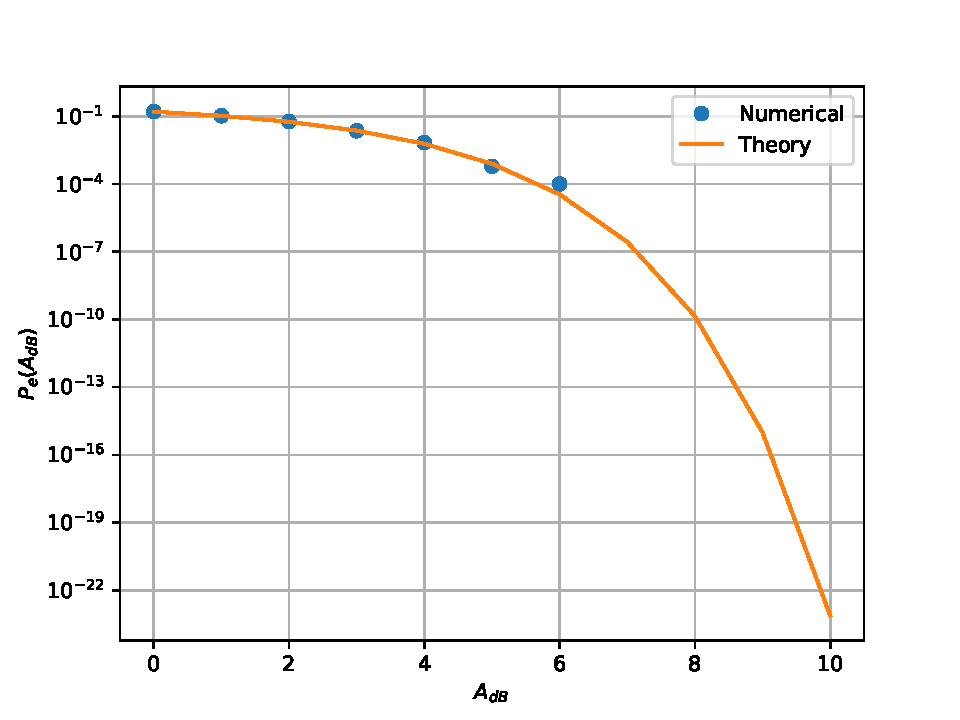
\includegraphics[scale=0.8]{chapter3/figs/bpsk_pe_snr.pdf}
\caption{$P_e$ versus $A$ plot}
\label{fig:bpsk_pe_snr}
\end{figure}
%
\item Now, consider a threshold $\delta$  while estimating $X$ from $Y$. Find the value of $\delta$ that maximizes the theoretical $P_e$.\\
\label{prob:bpsk_delta_equi}
\solution 




Let $\pr{0}$, $\pr{1}$ is a probability of transmitting bit zero and bit one;\\$P_{e|0}$,$P_{e|1}$is a probability of error when detecting bit zero and bit one.
\begin{equation}
	P_e = P_{e|0} \pr{0}+P_{e|1} \pr{1}
 \label{eq:error_prob}
\end{equation}
Let $V_0$,$V_1$ be a nominal signal voltage of bit zero and  one  signal at the transmitter.
$$
\begin{aligned}
& P(e \mid 0)=\int_ \delta^{\infty} \frac{1}{\sigma \sqrt{2 \pi}} \exp \left(-\left(\nu-V_0\right)^2 / 2 \sigma^2\right) d \nu \\
& P(e \mid 1)=\int_{-\infty}^ \delta \frac{1}{\sigma \sqrt{2 \pi}} \exp \left(-\left(\nu-V_1\right)^2 / 2 \sigma^2\right) d \nu
\end{aligned}
$$
where  $\delta$ is a detection threshold.
Differentiating $P(e)$ of  \eqref{eq:error_prob} w.r.t. $T$, we arrive at
$$
\begin{gathered}
-\pr{0} \frac{1}{\sigma \sqrt{2 \pi}} \exp \left(-\left( \delta-V_0\right)^2 / 2 \sigma^2\right)+ 
\\ \pr{1} \frac{1}{\sigma \sqrt{2 \pi}} \exp \left(-\left( \delta-V_1\right)^2 / 2 \sigma^2\right)
\end{gathered}
$$
To find an optimal threshold, we equate the above expression to zero:
$$
\begin{gathered}
\pr{0} \exp \left(-\frac{\left( \delta-V_0\right)^2}{2 \sigma^2}\right)=\pr{0} \exp \left(-\frac{\left( \delta-V_1\right)^2}{2 \sigma^2}\right) \\
 \delta=\frac{V_0+V_1}{2}+\sigma^2 \ln \left(\frac{\Pr{(1)}}{\pr{0}}\right)
\end{gathered}
$$
\begin{align*}
  \implies \Pr(1) = \Pr(0) = \frac{1}{2} \\
  \implies V_0=1,V_1=-1 \\
  \therefore  \delta =0 
\end{align*}
\item Repeat the above exercise when 
\label{prob:bpsk_decision_uneqi}
	\begin{align}
		p_{X}(0) = p
	\end{align}\\
\solution \begin{align}
	P_e &= (1-p)P_{e|1} + pP_{e|0}
\end{align}
From Above problem we know
$$
\begin{gathered}
 \delta=\frac{V_0+V_1}{2}+\sigma^2 \ln \left(\frac{P(1)}{P(0)}\right)\\
\delta =\ln \left(\frac{1-p}{p}\right)
\end{gathered}
$$
%\item Repeat the above exercise using the MAP criterion.\\
%\solution 
%The MAP rule can be stated as\\
%\begin{flalign}
%\label{eq:map_rule}
%\text{Set } \hat{x} &= x_i \text{ if}&\\ \nonumber
%p_X(x_k)p_Y(y|x_k) &\text{ is maximum for } k = i
%\end{flalign}
%For the case of BPSK, the point of equality between $p_X(x=1)p_Y(y|x=1)$ and $p_X(x=-1)p_Y(y|x=-1)$ is the optimum threshold. If this threshold is $\delta$, then
%\begin{flalign*}
%	pp_Y(y|x=1) > (1-p)p_Y(y|x=-1) &\text{ when } y > \delta&\\
%	pp_Y(y|x=1) < (1-p)p_Y(y|x=-1) &\text{ when } y < \delta 	
%\end{flalign*}
%The above inequalities can be visualized in \figref{fig:bpsk_map_density} for $p = 0.3$ and $A = 3$.
%\begin{figure}[H]
%\centering
%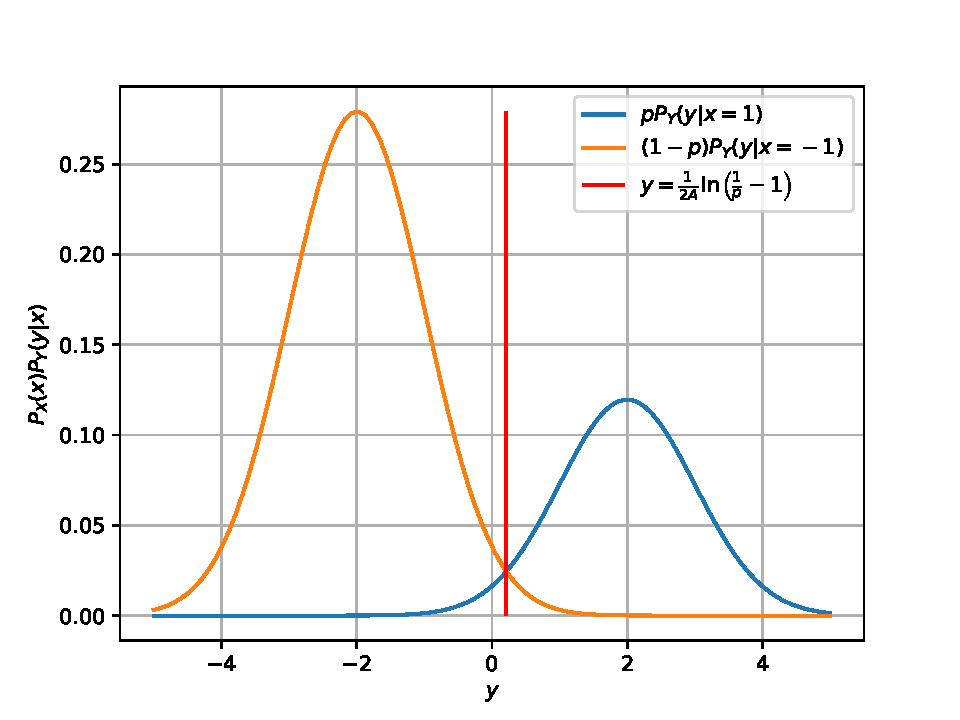
\includegraphics[width=\columnwidth]{chapter3/figs/bpsk_map_density.pdf}
%\caption{$p_X(X=x_i)p_Y(y|x=x_i)$ versus $y$ plot for $X \in \{-1,1\}$}
%\label{fig:bpsk_map_density}
%\end{figure}
%Given $Y=AX+N$ where $N \sim \gauss{0}{1}$, the optimum threshold is found as solution to the below equation
%\begin{equation}
%	p\exp\left(-\frac{(y_{eq}-A)^2}{2}\right) = (1-p)\exp\left(-\frac{(y_{eq}+A)^2}{2}\right)
%\end{equation}
%Solving for $y_{eq}$, we get
%\begin{equation}S
%	y_{eq} = \delta = \frac{1}{2A}\ln\left(\frac{1}{p}-1\right)
%\end{equation}
%which is same as $\delta$ obtained in problem \ref{prob:bpsk_decision_uneqi}
%
%\begin{lstlisting}
%		chapter3/codes/map.py	
%\end{lstlisting}
\end{enumerate}-
